
% LaTeX Beamer file automatically generated from DocOnce
% https://github.com/doconce/doconce

%-------------------- begin beamer-specific preamble ----------------------

\documentclass{beamer}

\usetheme{blue_shadow}
\usecolortheme{default}

% turn off the almost invisible, yet disturbing, navigation symbols:
\setbeamertemplate{navigation symbols}{}

% Examples on customization:
%\usecolortheme[named=RawSienna]{structure}
%\usetheme[height=7mm]{Rochester}
%\setbeamerfont{frametitle}{family=\rmfamily,shape=\itshape}
%\setbeamertemplate{items}[ball]
%\setbeamertemplate{blocks}[rounded][shadow=true]
%\useoutertheme{infolines}
%
%\usefonttheme{}
%\useinntertheme{}
%
%\setbeameroption{show notes}
%\setbeameroption{show notes on second screen=right}

% fine for B/W printing:
%\usecolortheme{seahorse}

\usepackage{pgf}
\usepackage{graphicx}
\usepackage{epsfig}
\usepackage{relsize}

\usepackage{fancybox}  % make sure fancybox is loaded before fancyvrb

\usepackage{fancyvrb}
%\usepackage{minted} % requires pygments and latex -shell-escape filename
%\usepackage{anslistings}
\usepackage{listingsutf8}

% Define colors
\definecolor{orange}{cmyk}{0,0.4,0.8,0.2}
\definecolor{tucorange}{rgb}{1.0,0.64,0}
\definecolor{darkorange}{rgb}{.71,0.21,0.01}
\definecolor{darkgreen}{rgb}{.12,.54,.11}
\definecolor{myteal}{rgb}{.26, .44, .56}
\definecolor{gray}{gray}{0.45}
\definecolor{mediumgray}{gray}{.8}
\definecolor{lightgray}{gray}{.95}
\definecolor{brown}{rgb}{0.54,0.27,0.07}
\definecolor{purple}{rgb}{0.5,0.0,0.5}
\definecolor{darkgray}{gray}{0.25}
\definecolor{darkblue}{rgb}{0,0.08,0.45}
\definecolor{darkblue2}{rgb}{0,0,0.8}
\definecolor{lightred}{rgb}{1.0,0.39,0.28}
\definecolor{lightgreen}{rgb}{0.48,0.99,0.0}
\definecolor{lightblue}{rgb}{0.53,0.81,0.92}
\definecolor{lightblue2}{rgb}{0.3,0.3,1.0}
\definecolor{lightpurple}{rgb}{0.87,0.63,0.87}
\definecolor{lightcyan}{rgb}{0.5,1.0,0.83}

\colorlet{comment_green}{green!50!black}
\colorlet{string_red}{red!60!black}
\colorlet{keyword_pink}{magenta!70!black}
\colorlet{indendifier_green}{green!70!white}

% Backgrounds for code
\definecolor{cbg_gray}{rgb}{.95, .95, .95}
\definecolor{bar_gray}{rgb}{.92, .92, .92}

\definecolor{cbg_yellowgray}{rgb}{.95, .95, .85}
\definecolor{bar_yellowgray}{rgb}{.95, .95, .65}

\colorlet{cbg_yellow2}{yellow!10}
\colorlet{bar_yellow2}{yellow!20}

\definecolor{cbg_yellow1}{rgb}{.98, .98, 0.8}
\definecolor{bar_yellow1}{rgb}{.98, .98, 0.4}

\definecolor{cbg_red1}{rgb}{1, 0.85, 0.85}
\definecolor{bar_red1}{rgb}{1, 0.75, 0.85}

\definecolor{cbg_blue1}{rgb}{0.87843, 0.95686, 1.0}
\definecolor{bar_blue1}{rgb}{0.7,     0.95686, 1}

\usepackage{listingsutf8}

% Common lstlisting parameters

\usepackage{calc}
\newlength{\lstboxwidth}  % width of lst box
\newlength{\framethickness}
\setlength{\framethickness}{0.5mm}
% for frame=trbl and a framerule that has significant size, set
% xleftmargin=5mm and xrightmargin=5mm.

\lstset{
  basicstyle=\small \ttfamily,
  breaklines=false,          % break/wrap lines
  breakatwhitespace=true,    % let linebreaks happen at whitespace
  breakindent=40pt,
  tab=,
  tabsize=4,                 % tab means 4 spaces
  %belowskip=\smallskipamount,  % space between code and text below
  xleftmargin=2mm,           % indentation of code frame
  xrightmargin=0mm,
  framexleftmargin=2mm,      % add frame space to the left of the code box
  %numbers=left,             % put line numbers on the left
  %stepnumber=2,             % stepnumber=1 numbers each line, =n every n lines
  framerule=\framethickness, % thickness of frame
  aboveskip=2ex,             % vertical space above code frame
  showstringspaces=false,    % show spaces in strings with an underscore
  showspaces=false,          % show spaces with an underscore
  showtabs=false,
  keepspaces=true,
  columns=fullflexible,      % tighter character kerning, like verb
  escapeinside={(*@}{@*)},   % (*@ \pause @*) in slides and math in code blocks
  extendedchars=\true,       % allows non-ascii chars, does not work with utf-8
}

% Internally defined styles for lstlisting

% Use this one without additional background color
\lstdefinestyle{yellow2_fb}{         % approx same colors as in the FEniCS book
frame=tb,                            % top+bottom frame
rulecolor=\color{black},             % frame color
framerule=0.4pt,                     % thickness of frame
backgroundcolor=\color{yellow!10},
keywordstyle=\color{blue}\bfseries,
commentstyle=\color{comment_green}\slshape,
stringstyle=\color{string_red},
identifierstyle=\color{darkorange},
}

\lstdefinestyle{simple}{
commentstyle={},
}

% end of custom lstdefinestyles

\usepackage{amsmath,amssymb,bm}
%\usepackage[latin1]{inputenc}
\usepackage[T1]{fontenc}
\usepackage[utf8]{inputenc}
\usepackage{colortbl}
\usepackage[english]{babel}
\usepackage{tikz}
\usepackage{framed}
% Use some nice templates
\beamertemplatetransparentcovereddynamic

% --- begin table of contents based on sections ---
% Delete this, if you do not want the table of contents to pop up at
% the beginning of each section:
% (Only section headings can enter the table of contents in Beamer
% slides generated from DocOnce source, while subsections are used
% for the title in ordinary slides.)
\AtBeginSection[]
{
  \begin{frame}<beamer>[plain]
  \frametitle{}
  %\frametitle{Outline}
  \tableofcontents[currentsection]
  \end{frame}
}
% --- end table of contents based on sections ---

% If you wish to uncover everything in a step-wise fashion, uncomment
% the following command:

%\beamerdefaultoverlayspecification{<+->}

\newcommand{\shortinlinecomment}[3]{\note{\textbf{#1}: #2}}
\newcommand{\longinlinecomment}[3]{\shortinlinecomment{#1}{#2}{#3}}

\definecolor{linkcolor}{rgb}{0,0,0.4}
\hypersetup{
    colorlinks=true,
    linkcolor=linkcolor,
    urlcolor=linkcolor,
    pdfmenubar=true,
    pdftoolbar=true,
    bookmarksdepth=3
    }
\setlength{\parskip}{7pt}  % {1em}

\newenvironment{doconceexercise}{}{}
\newcounter{doconceexercisecounter}
\newenvironment{doconce:movie}{}{}
\newcounter{doconce:movie:counter}

\newcommand{\subex}[1]{\noindent\textbf{#1}}  % for subexercises: a), b), etc

%-------------------- end beamer-specific preamble ----------------------

% Add user's preamble




% insert custom LaTeX commands...

\raggedbottom
\makeindex

%-------------------- end preamble ----------------------

\begin{document}

% matching end for #ifdef PREAMBLE
% #endif

\newcommand{\exercisesection}[1]{\subsection*{#1}}

\input{newcommands_bfmath}
\input{newcommands_replace}


% ------------------- main content ----------------------



% ----------------- title -------------------------

\title{Document for Testing Some Basic and Some Challenging Constructs in DocOnce Slides}

% ----------------- author(s) -------------------------

\author{Hans Petter Langtangen\inst{1,2}}
\institute{Simula Research Laboratory\inst{1}
\and
University of Oslo\inst{2}}
% ----------------- end author(s) -------------------------

\date{Jan 32, 2100
% <optional titlepage figure>
% <optional copyright>
}

\begin{frame}[plain,fragile]
\titlepage
\end{frame}

\section[First]{This is the first section}

\begin{frame}[plain,fragile]
\frametitle{Figure and bullet list}

\begin{columns}
\column{0.6\textwidth}
\pause
\begin{block}{Title with comma, and brackets: $[a,b]$ }
\footnotesize

\begin{itemize}
  \item Here is a \emph{wave signal} $f(x-ct)$

  \item It moves with velocity $c$

  \item But here it is just a figure
\end{itemize}

\noindent
\end{block}

\column{0.4\textwidth}
\begin{block}{}

\vspace{6mm}

% inline figure
\centerline{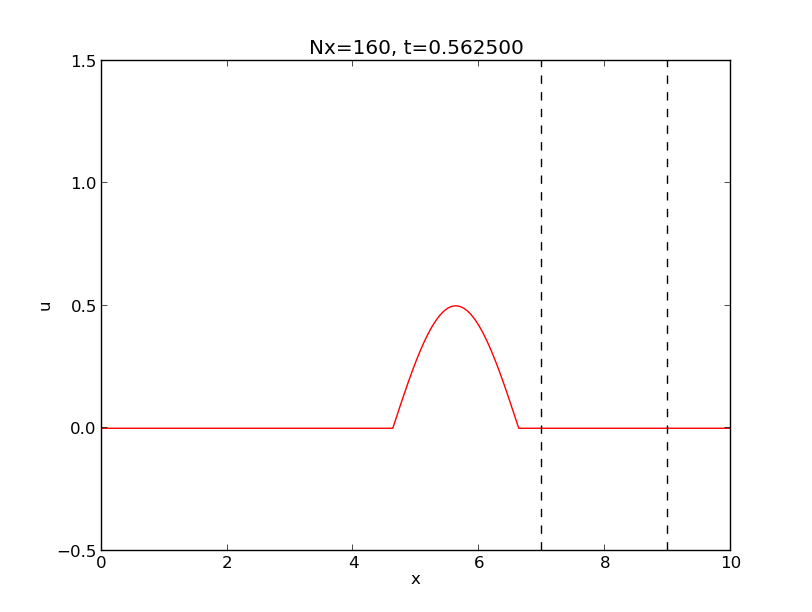
\includegraphics[width=0.7\linewidth]{testfigs/wave1D.png}}

\vspace{6mm}

\end{block}

\end{columns}
\end{frame}

\begin{frame}[plain,fragile]
\frametitle{Slide with pop-ups in red and notes}

\shortinlinecomment{hpl 1}{ Comments are typeset as usual in DocOnce. }{ Comments are typeset as }

\pause
Here we have a paragraph to pop up in red.\\
And a line more

\note{
One can also have ordinary notes.
Over multiple lines.
}
\end{frame}

\begin{frame}[plain,fragile]
\frametitle{A {\LaTeX} document}

\pause
\begin{lstlisting}[language=TeX,style=yellow2_fb]
\documentclass[11pt]{article}
\usepackage{fancyvrb}
\begin{document}

\title{Here goes the title...}
\author{John Doe \and
Jane Doe\footnote{\texttt{jane.doe@cyber.net}.}}
\date{\today}
\maketitle

\end{lstlisting}

\pause
\begin{block}{Notice}
{\LaTeX} has a lot of backslashes.
\end{block}

\pause
\begin{lstlisting}[language=TeX,style=yellow2_fb]
\section{Heading}
bla-bla
\end{document}

\end{lstlisting}
\end{frame}

\begin{frame}[plain,fragile]
\frametitle{An HTML document}

\begin{lstlisting}[language=html,style=yellow2_fb]
<html><head></head><body bgcolor="red">
<title>Here goes the title...<title>
<h1>Section heading</h1>
</body>
</html>

\end{lstlisting}
\end{frame}

\section{Second section}

\begin{frame}[plain,fragile]
\frametitle{Second section}


\begin{block}{}

\vspace{6mm}

% inline figure
\centerline{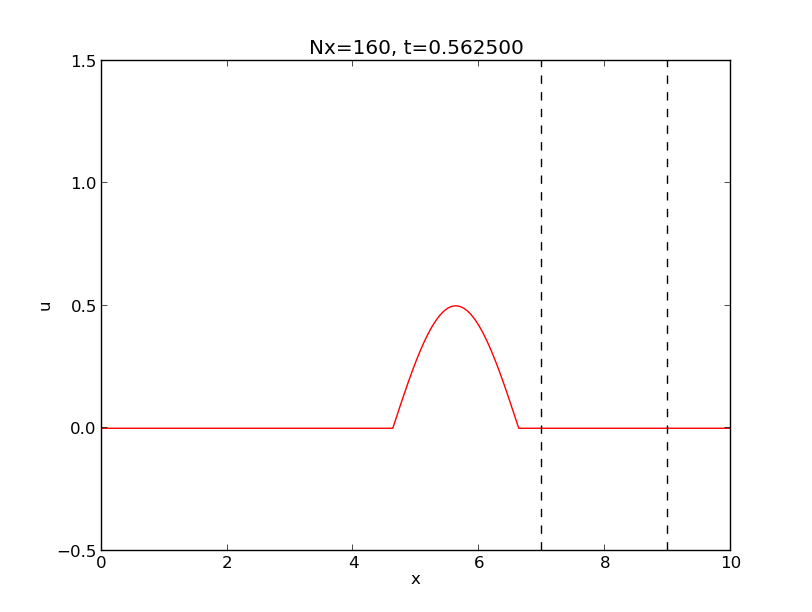
\includegraphics[width=0.8\linewidth]{testfigs/wave1D.png}}

\vspace{6mm}

\end{block}


\end{frame}

\begin{frame}[plain,fragile]
\frametitle{Some math and computer code}

\begin{block}{A simple, mathematical formula where $t\in [0,\pi]$: }
\[ f(x,y,t) = e^{-xt}\sin\pi y \]
\end{block}

\begin{block}{Bash demanded more of DocOnce than Python, so let's do Bash: }
First, inline \Verb@$? != 0@, then comments with dollar variables (and minted
style):







\begin{lstlisting}[language=bash,style=yellow2_fb]
var=10
# $1, $2, ... are command-line args
if [ $? -eq 0 ]; then   # $? reflects success or not
  echo "Great!"
fi

\end{lstlisting}

\end{block}
\end{frame}

\begin{frame}[plain,fragile]
\frametitle{Pop ups inside code blocks (for Beamer slides only)}

\begin{lstlisting}[language=python,style=yellow2_fb]
def f(x):
    return 42 + x

(*@\pause@*)
def g(x):
    return f(42)

(*@\pause@*)
print(g(13))

\end{lstlisting}
\end{frame}

\begin{frame}[plain,fragile]
\frametitle{Various admon blocks}

Can use admons to simulate blocks:

\pause
\begin{block}{Key PDE (with large title and math font): }
\large

\[ \frac{\partial u}{\partial t} = \nabla^2 u \]
\end{block}

\pause
\begin{block}{}
Just some block with text and a conclusion that something is important.
This one pops up after the rest of the slide.
\end{block}

\pause
\begin{block}{Warning}
\footnotesize

Can use, e.g., a warning admon to have my own notes, preferably
inside preprocess/mako if statements to turn notes on and off.
This one is typeset in a small font and with the default
title (Warning) since no title is specified.
\end{block}
\end{frame}

\end{document}
